Esta sección ofrece una visión general de los distintos grupos funcionales y funcionalidades concretas que ofrece la aplicación desarrollada. Además, profundiza en aspectos concretos, como la gestión de la visibilidad de recursos.

La sección se divide en dos partes introductorias, que ponen en contexto la aplicación y describen los tipos de usuarios que participan en ella, y tres secciones detallando las funcionalidades básicas, avanzadas esenciales, y avanzadas opcionales. Adicionalmente, para poder ofrecer una visión general, sin listar todas las funcionalidades de la aplicación, se han descrito 5 unidades funcionales, en las que se agrupan las distintas funcionalidades de la aplicación. La discusión durante estas tres secciones estará centrada en estas unidades funcionales, que se describen a continuación:
\begin{enumerate}
    \item \textbf{Gestión de Actividades:} agrupa las funcionalidades que toman como base una actividad. 
    \item \textbf{Gestión de Rutas:} agrupa las funcionalidades que toman como base una ruta. 
    \item \textbf{Gestión de Murales:} agrupa las funcionalidades que toman como base un mural 
    \item \textbf{Gestión de Usuarios:} agrupa las funcionalidades que toman como base un usuario. 
    \item \textbf{Gestión de visibilidad:} agrupa las operaciones que actúan sobre la visibilidad de los distintos recursos. 
\end{enumerate}


\section{Visión general de la aplicación}
La aplicación desarrollada tiene como funcionalidad principal permitir a los usuarios subir actividades para su estudio y comparación con otras actividades similares, para poder analizar su desempeño en actividades concretas o ver su evolución a lo largo del tiempo.

Además de estas funcionalidades, se ofrece un aspecto social mediante murales. Estos son grupos donde varios usuarios pueden compartir rutas y actividades, comparar su desempeño con el de otros, y ver métricas colectivas.

\noindent Es importante dejar claro qué funcionalidades la aplicación NO busca cumplir:
\begin{itemize}
    \item No permite la grabación de actividades nuevas. Pretende ser una herramienta exclusivamente de análisis y comparación de actividades. La grabación de actividades y generación de archivos GPX se delega en otros servicios.
    \item No permite interacción entre usuarios más allá de la pertenencia a un mural común. La única herramienta social son los murales. No se gestiona una red de "amigos" ni "usuarios similares", ni se ofrecen funcionalidades para la comunicación directa entre dos usuarios.
\end{itemize}

Esta sección no ofrece un listado completo de funcionalidades, sino una visión más general. El listado completo de funcionalidades se incluye en el Anexo \ref{anexo:funcionalidades-detalladas}

Adicionalmente, se pueden visualizar las distintas funcionalidades mediante un vídeo demostrativo, disponible en el siguiente enlace: \href{https://youtu.be/RNXF-EBCMn4}{\uline{Demo de las funcionalidades de la aplicación}\footnote{\url{https://youtu.be/RNXF-EBCMn4}}}

\section{Tipos de usuario}
Se consideran 3 tipos de usuario principales:
\begin{itemize}
    \item Usuario anónimo: cualquier usuario que no ha iniciado sesión en el sistema. Actualmente no tiene acceso a ninguna funcionalidad. Se plantea hacer accesibles las funcionalidades de estudio y comparación de actividades para usuarios anónimos como mejora a futuro.
    \item Usuario autenticado: el usuario básico, con identidad definida. Puede crear y acceder a rutas, actividades, y murales, y tiene control sobre entidades que haya creado.
    \item Usuario administrador: Supervisor del sistema, encargado de asegurar el uso adecuado de la aplicación. Tiene la capacidad de eliminar recursos públicos.
\end{itemize}

\section{Funcionalidades básicas}
Las funcionalidades básicas son aquellas que se consideran esenciales para el funcionamiento mínimo de la aplicación. Incluyen las operaciones de creación, consulta, edición, y eliminación de usuarios, actividades, rutas, y murales, así como alguna otra funcionalidad adicional.

\subsection{Gestión de actividades}
Las funcionalidades básicas de este grupo funcional incluyen crear, eliminar, y visualizar actividades, entre otras. Las actividades son la entidad central de la aplicación, siendo utilizadas por las otras entidades, y siendo el recurso con el que más interactuarán los usuarios. Como tal, tienen un repertorio más amplio de funcionalidades que otras entidades. 

Los usuarios pueden ver un listado de sus actividades, y seleccionar una para estudiar más en detalle. Cuando el usuario decida estudiar una actividad concreta, visualizará tanto información básica (como el nombre y fecha de la actividad), como métricas y otra información calculada (como ritmo medio y distancia total). Además, la aplicación calcula ciertas métricas estadísticas de interés, y que evalúan la distribución y calidad de los valores obtenidos o calculados. Por ejemplo, se calcula y muestra la media, los percentiles 25, 50, y 75, el rango intercuartil, el porcentaje de valores considerados anómalos o erróneos, y la desviación media. También se permite al usuario definir un valor objetivo para la métrica seleccionada, junto con límites superior e inferior, y se muestra el porcentaje de valores de la métrica seleccionada que caen en cada división definida por el objetivo y los límites.

Por ejemplo, si mi objetivo es mantener un ritmo medio de 6:00 minutos por kilómetro, puedo determinar 6:00 como objetivo, 5:50 como límite inferior, y 6:10 como límite superior, y la aplicación me mostrará el porcentaje de valores por debajo de 5:50, entre 5:50 y 6:00, entre 6:00 y 6:10, y por encima de 6:00.

El objetivo de todas estas funcionalidades es que los usuarios puedan estudiar en detalle su desempeño, principalmente mediante el estudio del ritmo. Sin embargo, estas funcionalidades no están disponibles únicamente para el ritmo, sino que también estarán disponibles para otras métricas como las pulsaciones o la cadencia de zancada. Estas medidas estadísticas son de utilidad porque informan al usuario de su consistencia, y le permiten ver cuánto se acerca a sus objetivos, permitiéndose cierto margen de error. El rango intercuartil informa sobre lo agrupados que estén los valores, indicando lo estable que ha sido el ritmo. El objetivo y límites permiten saber durante qué porcentaje de la actividad el usuario ha mantenido su ritmo en un rango determinado. El porcentaje de valores erróneos informa sobre la calidad de los datos, y la desviación media, junto con los percentiles y la media, son valores de interés general. 

Adicionalmente, la aplicación ofrece una manera de visualizar todos estos datos mediante dos tipos de gráficos: 
\begin{itemize}
    \item Gráfico de líneas: muestra una métrica (ritmo, cadencia, pulsaciones) en el eje vertical, frente al tiempo transcurrido desde el inicio de la actividad en el eje horizontal.
    \item Histograma: permite visualizar la distribución de los valores obtenidos para la métrica seleccionada. El objetivo es poder ver fácilmente cómo están distribuidos los valores: si siguen una distribución normal o no, si la distribución pone más peso antes o después de la media, etc. 
\end{itemize}
Estos gráficos ofrecen ciertas funcionalidades de personalización, como:
\begin{enumerate}
    \item Mostrar la media y los percentiles (25\%, 50\%, 75\%) en la gráfica de líneas.
    \item Mostrar y modificar los valores de los límites definidos por el usuario en la gráfica de líneas.
    \item Modificar el número de particiones del histograma.
\end{enumerate}

Otra funcionalidad esencial en este grupo funcional es el poder visualizar la actividad en un mapa, de forma que los usuarios puedan visualizar la ruta tomada. 

Las figuras \ref{fig:resumen_actividad} y \ref{fig:func_bas_estudio_act} muestran algunas de las funcionalidades discutidas, siendo estas, principalmente, la visualización de datos y métricas sobre las actividades, visualización de la actividad en el mapa, y visualización de la actividad en gráficos configurables.
\begin{figure}[H]
    \centering
    \begin{minipage}{0.48\linewidth}
        \centering
        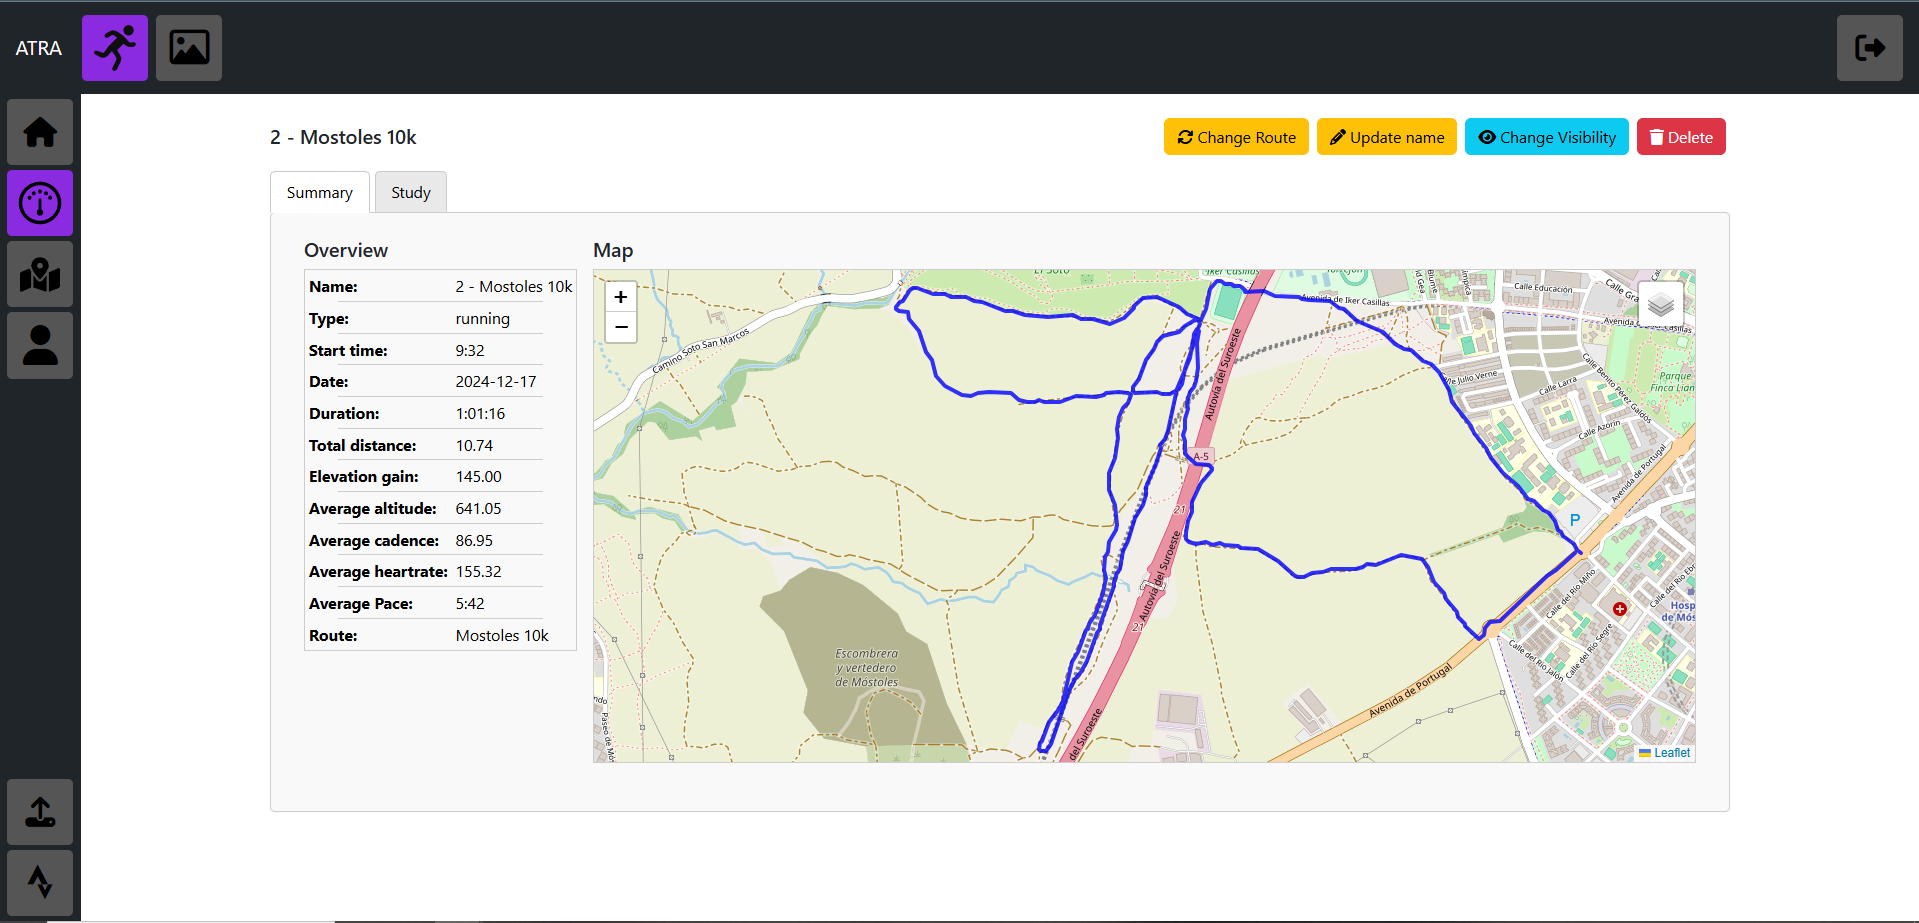
\includegraphics[width=\linewidth]{img/resumen_actividad.png}
        \caption{Visualización de mapa y resumen de actividad}
        \label{fig:resumen_actividad}
    \end{minipage}
    \hfill
    \begin{minipage}{0.48\linewidth}
        \centering
        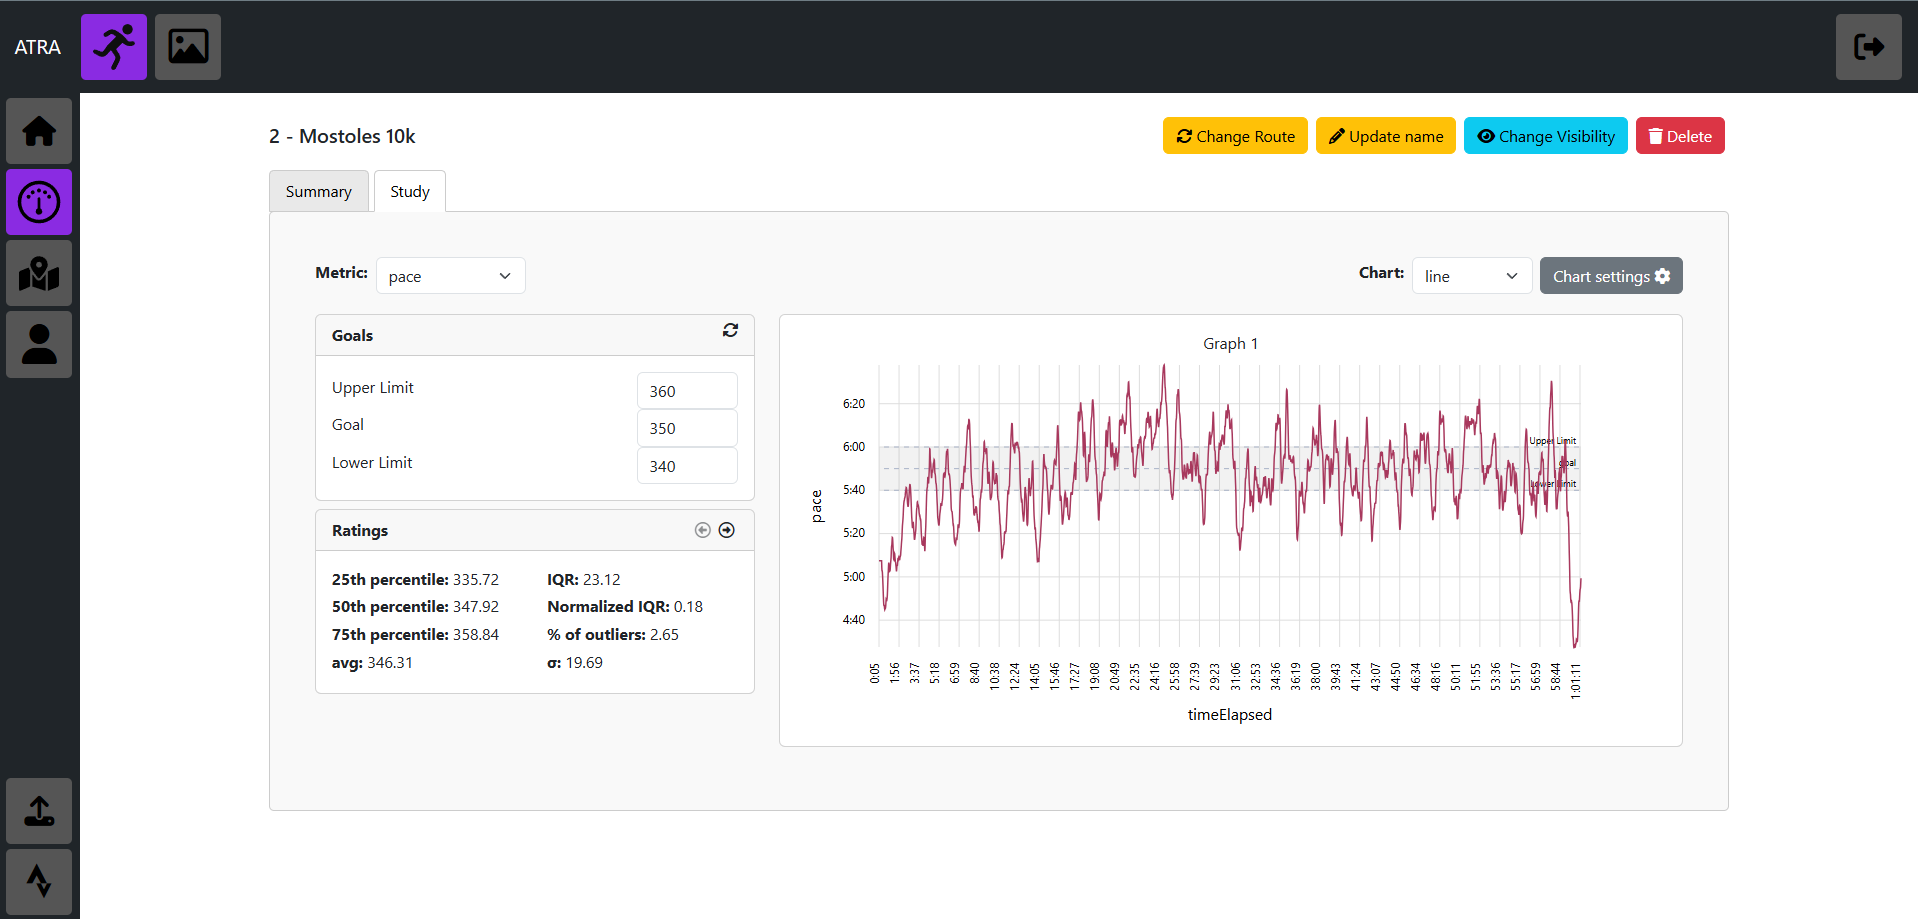
\includegraphics[width=\linewidth]{img/func_bas_estudio_act.png}
        \caption{Visualización de métricas de una actividad}
        \label{fig:func_bas_estudio_act}
    \end{minipage}
\end{figure}

En resumen, se cubren las operaciones básicas de creación, eliminación y visualización, junto con otras específicas a las actividades, como el cálculo de métricas, la visualización de datos en gráficas, y la visualización de la actividad en un mapa.

\subsection{Gestión de Rutas}
Las funcionalidades básicas de este grupo funcional incluyen crear, visualizar, editar, y eliminar rutas. Las rutas son un recurso auxiliar, que permite agrupar varias actividades que hayan seguido el mismo camino, para poder ser visualizadas o estudiadas en conjunto.

Para crear una ruta se debe partir de una actividad. Teniendo una actividad seleccionada que no tenga ruta asignada, existe un botón para crear una ruta a partir de esa actividad. Cuando el usuario le haga click, se muestra un formulario permitiendo modificar el nombre, descripción, distancia total y elevación acumulada. Se toma como valores por defecto los de la actividad seleccionada, pero permiten modificación, ya que varias actividades en una misma ruta a veces tienen valores ligeramente distintos. Cuando el usuario decida crear la ruta, se le da la opción de visualizarla.

En cualquier momento, el usuario puede acceder a un listado de rutas, a través del cual podrá seleccionar una ruta para ver sus datos en detalle o realizar operaciones sobre ella. Cuando seleccione una ruta, se le muestra un listado de las actividades que forman parte de ella, junto con un mapa, y los datos especificados al crearla. Además, el usuario tiene acceso a una serie de botones para eliminar la ruta, modificar su visibilidad, y añadir nuevas actividades o quitar actividades existentes. Se pueden observar estas funcionalidades en la figura \ref{fig:func_bas_ruta}

\begin{figure}[H]
    \centering
    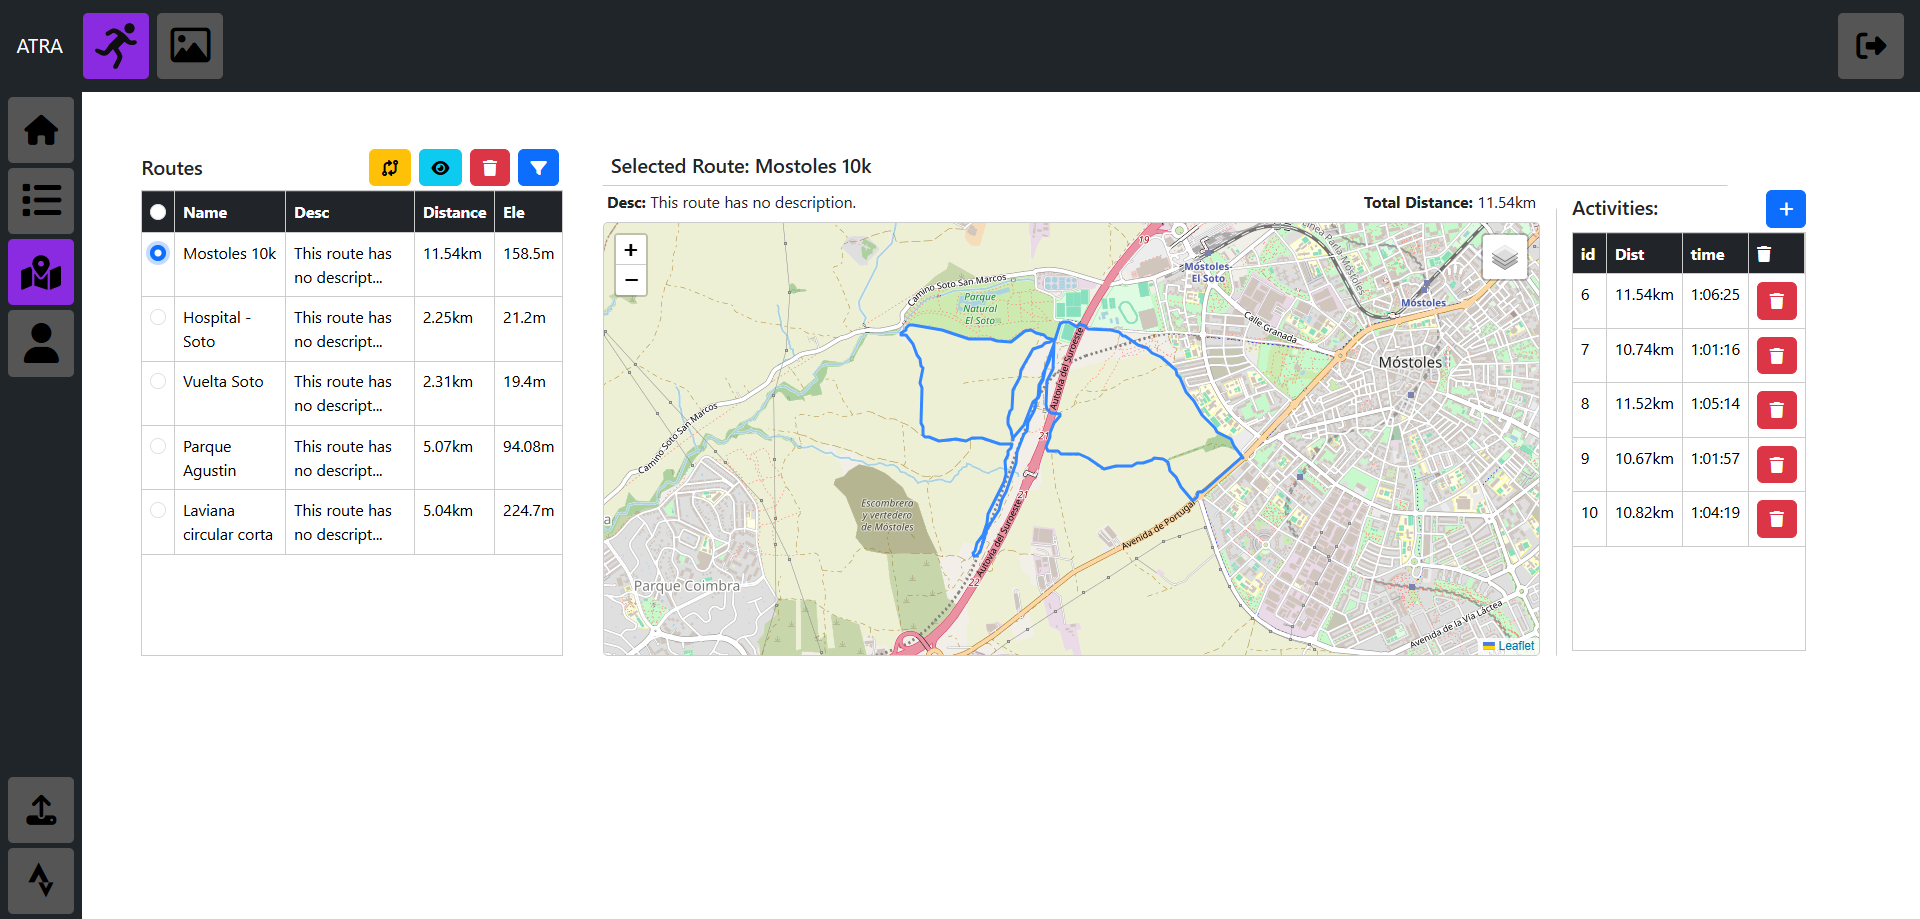
\includegraphics[width=1\linewidth]{img/func_bas_ruta.png}
    \caption{Listado de rutas y visualización de ruta seleccionada}
    \label{fig:func_bas_ruta}
\end{figure}

\subsection{Gestión de Murales}
Las funcionalidades básicas en este grupo funcional incluyen crear, modificar, visualizar, y eliminar murales, así como unirse a ellos. Los murales son el principal recurso social de la aplicación, permitiendo a los usuarios compartir sus actividades y rutas creadas con amigos, para ver su actividad, o comparar su desempeño en las mismas rutas.

\begin{figure}[H]
    \centering
    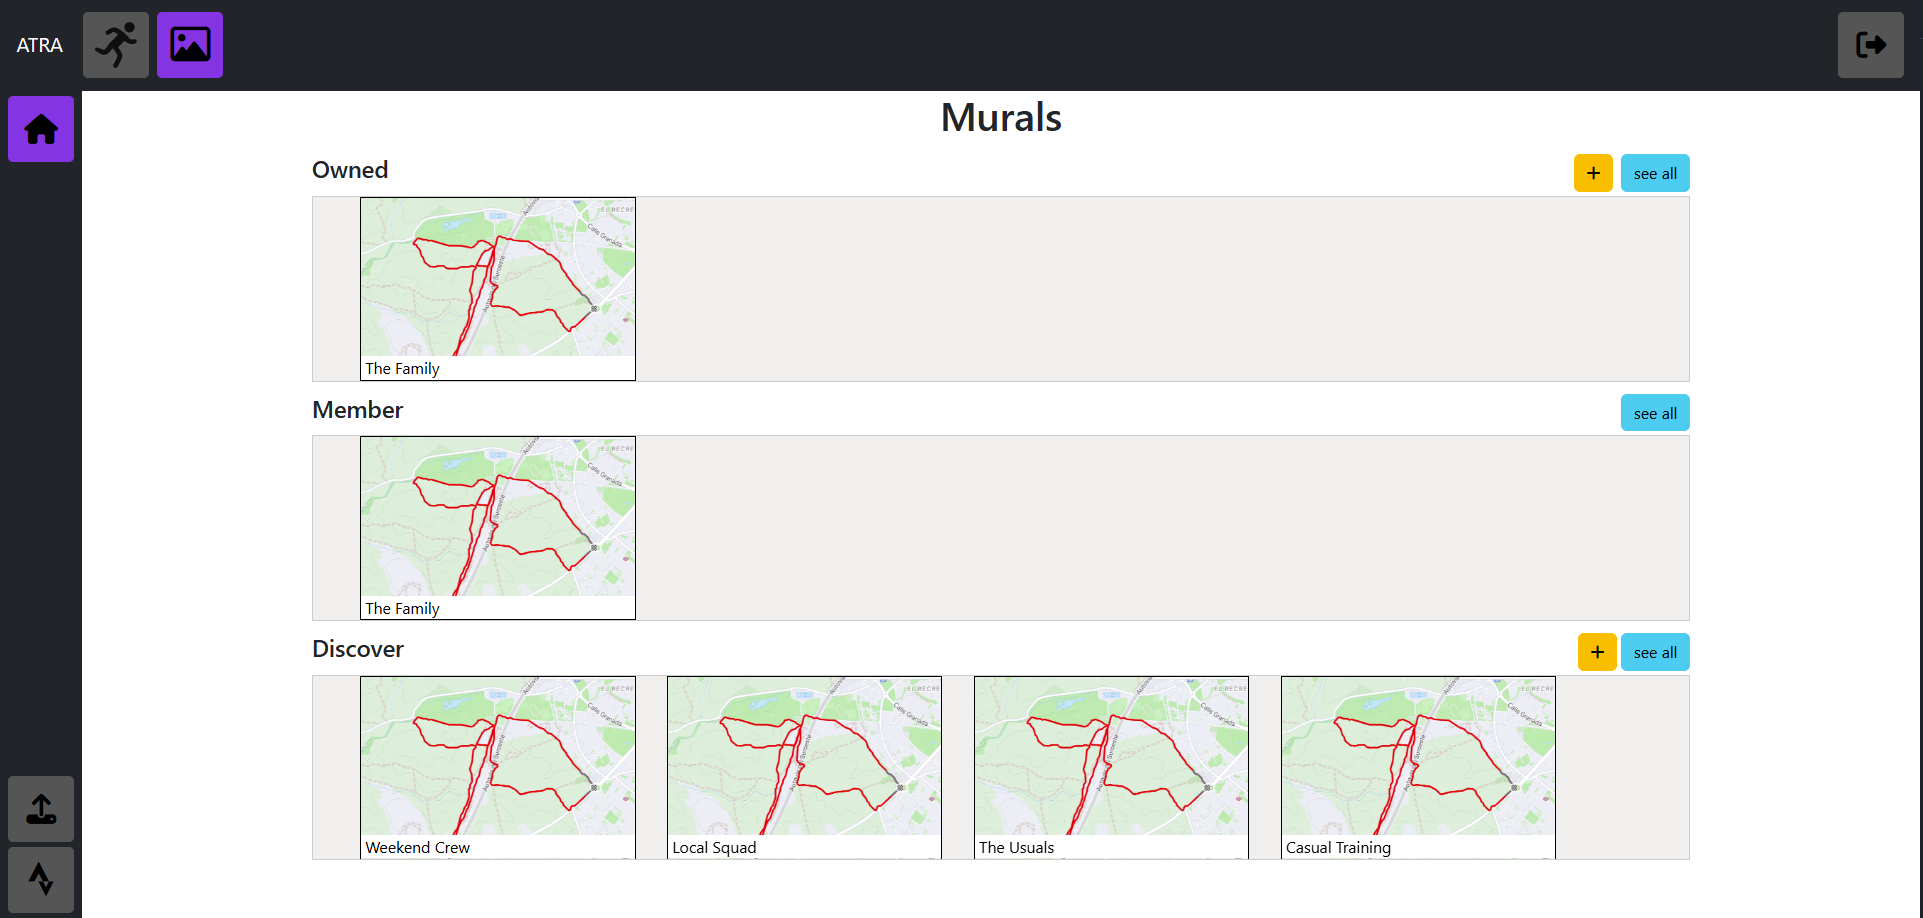
\includegraphics[width=0.75\linewidth]{img/lista_murales.png}
    \caption{Listado de murales por categorías}
    \label{fig:lista_murales}
\end{figure}

Cuando el usuario accede a la página de murales, se le presentan tres listas (visibles en la figura \ref{fig:lista_murales}), mostrando: murales creados, murales de los que es miembro, y murales en los que no es miembro. El usuario puede acceder a cualquier mural en el que es miembro, crear un nuevo mural, o unirse a un mural de dos formas distintas. Puede unirse a un mural con el código único a ese mural (a través del botón + en la sección discover), o seleccionando el mural en la lista de murales a los que no pertenece. Además, tiene disponible un botón para ver el listado completo de murales en cada categoría, ya que esta pantalla muestra una selección limitada de murales.

Desde esta pantalla, el usuario puede crear un mural nuevo, pulsando sobre el botón + amarillo encima de la lista \textit{Owned}. Al hacerlo, se le muestra un modal en el que debe rellenar los datos del mural. Deberá aportar nombre, descripción, visibilidad, imagen de miniatura (visible en la lista), e imagen de \textit{banner} (visible en el detalle del mural, figura \ref{fig:mural_dashboard}). Estas imágenes deben tener una relación de aspecto de 4:3 para la miniatura, y 5:1 para el \textit{banner}. Si se introducen imágenes con relaciones de aspecto erróneas, la aplicación no permitirá crear el mural.

\begin{figure}[H]
    \centering
    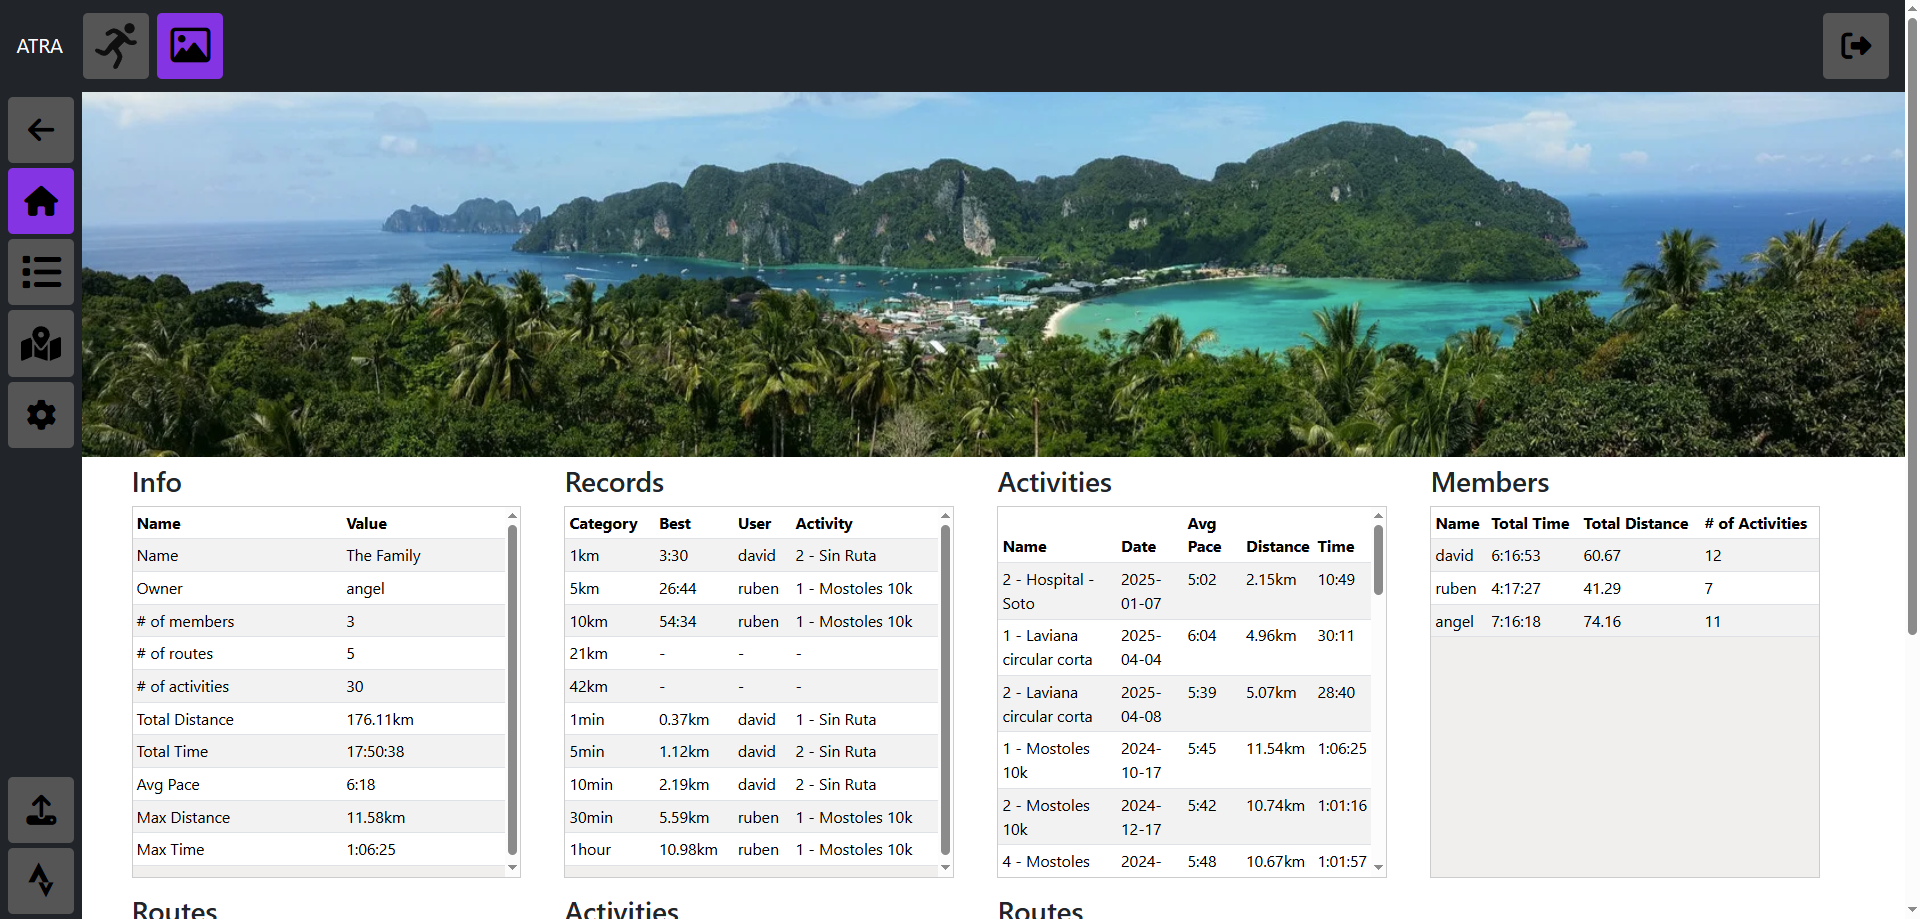
\includegraphics[width=0.75\linewidth]{img/mural_dashboard.png}
    \caption{Dashboard del mural}
    \label{fig:mural_dashboard}
\end{figure}

Cuando el usuario decida acceder a un mural, aterrizará en el \textit{dashboard} del mural (representado en la figura \ref{fig:mural_dashboard},) que le muestra información general del mural, como cuantos miembros, actividades, y rutas tiene, el tiempo y distancia total de todas las actividades en el mural, y un listado de récords, mostrando marcas como el menor tiempo en recorrer un kilómetro, o la máxima distancia cubierta en una hora.

Desde el \textit{dashboard} también puede ver un listado de miembros, rutas, y actividades en el mural. Si hace click sobre una actividad o ruta, podrá ver la información de la misma. Alternativamente, puede navegar a través del menú lateral para acceder al listado completo de actividades o rutas a las que tiene acceso el mural.

\begin{figure}[H]
    \centering
    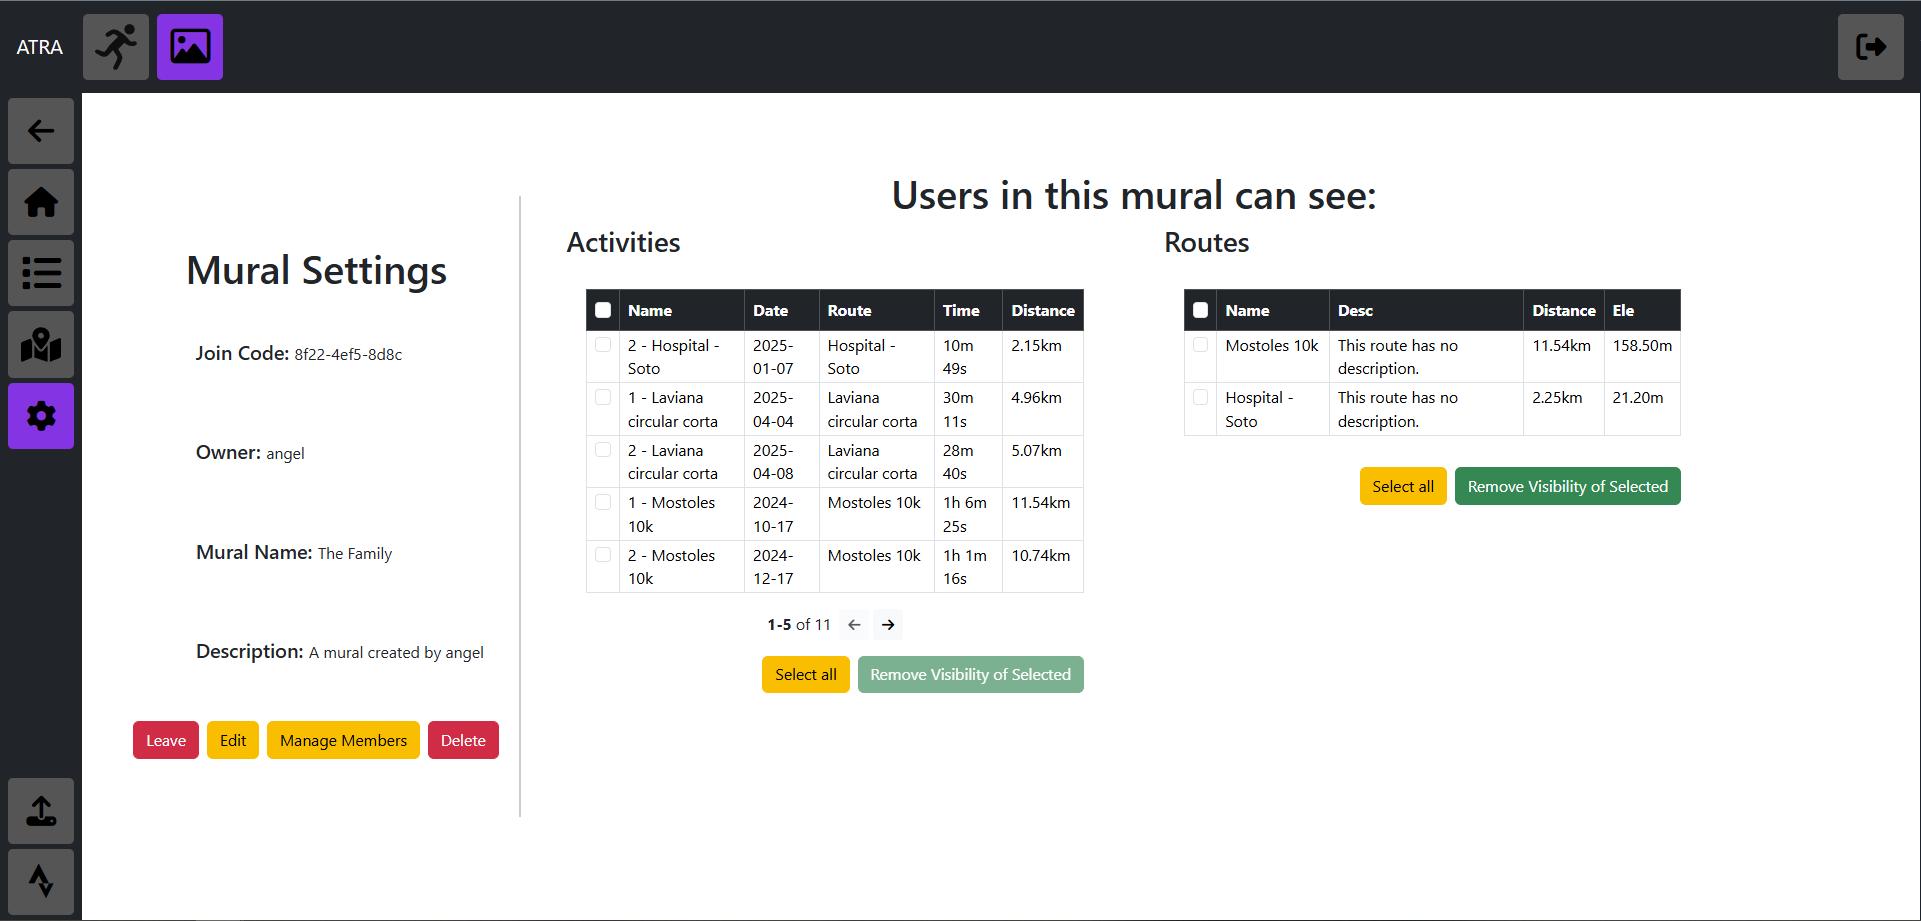
\includegraphics[width=0.75\linewidth]{img/mural_config.png}
    \caption{Pantalla de Configuración del Mural}
    \label{fig:mural_config}
\end{figure}

Por último, existe una pantalla de configuración, dentro de la cual el usuario puede gestionar a qué rutas y actividades propias tiene acceso el mural, y dispone de un un botón con el que abandonar el mural. Adicionalmente, si el usuario resulta ser el propietario del mural, puede editar la información del mural desde esta pantalla, pudiendo cambiar datos genéricos como el nombre, la descripción, la miniatura, o el \textit{banner}, así como hacer gestiones más avanzadas, como echar a usuarios. Cabe destacar que el propietario del mural no podrá irse del mismo, ya que la funcionalidad de traspasar propiedad es más avanzada. En esta etapa, si el propietario quiere dejar el mural, deberá eliminarlo.

\subsection{Gestión de Usuarios}
Las funcionalidades básicas de este grupo funcional incluyen crear y eliminar usuarios, así como iniciar y cerrar sesión en un usuario creado. Los usuarios representan a las personas que interactúan con el sistema y cuyos datos se almacenan en la base de datos.

Para poder acceder al sistema y usar las funcionalidades, los usuarios deben autenticarse, es decir, iniciar sesión como un usuario registrado en el sistema. En caso de no tener un usuario asignado, este puede ser creado aportando un nombre de usuario y una contraseña. El inicio de sesión y registro de un nuevo usuario son las únicas funcionalidades accesibles sin iniciar sesión. 

Cuando el usuario inicie sesión, atteriza en un \textit{dashboard}, muy similar al que se visualiza al acceder a un mural. Este \textit{dashboard} consiste en varios paneles que presentan cierta información. La figura \ref{fig:user_dashboard} muestra un ejemplo del \textit{dashboard} del usuario.

\begin{figure}[H]
    \centering
    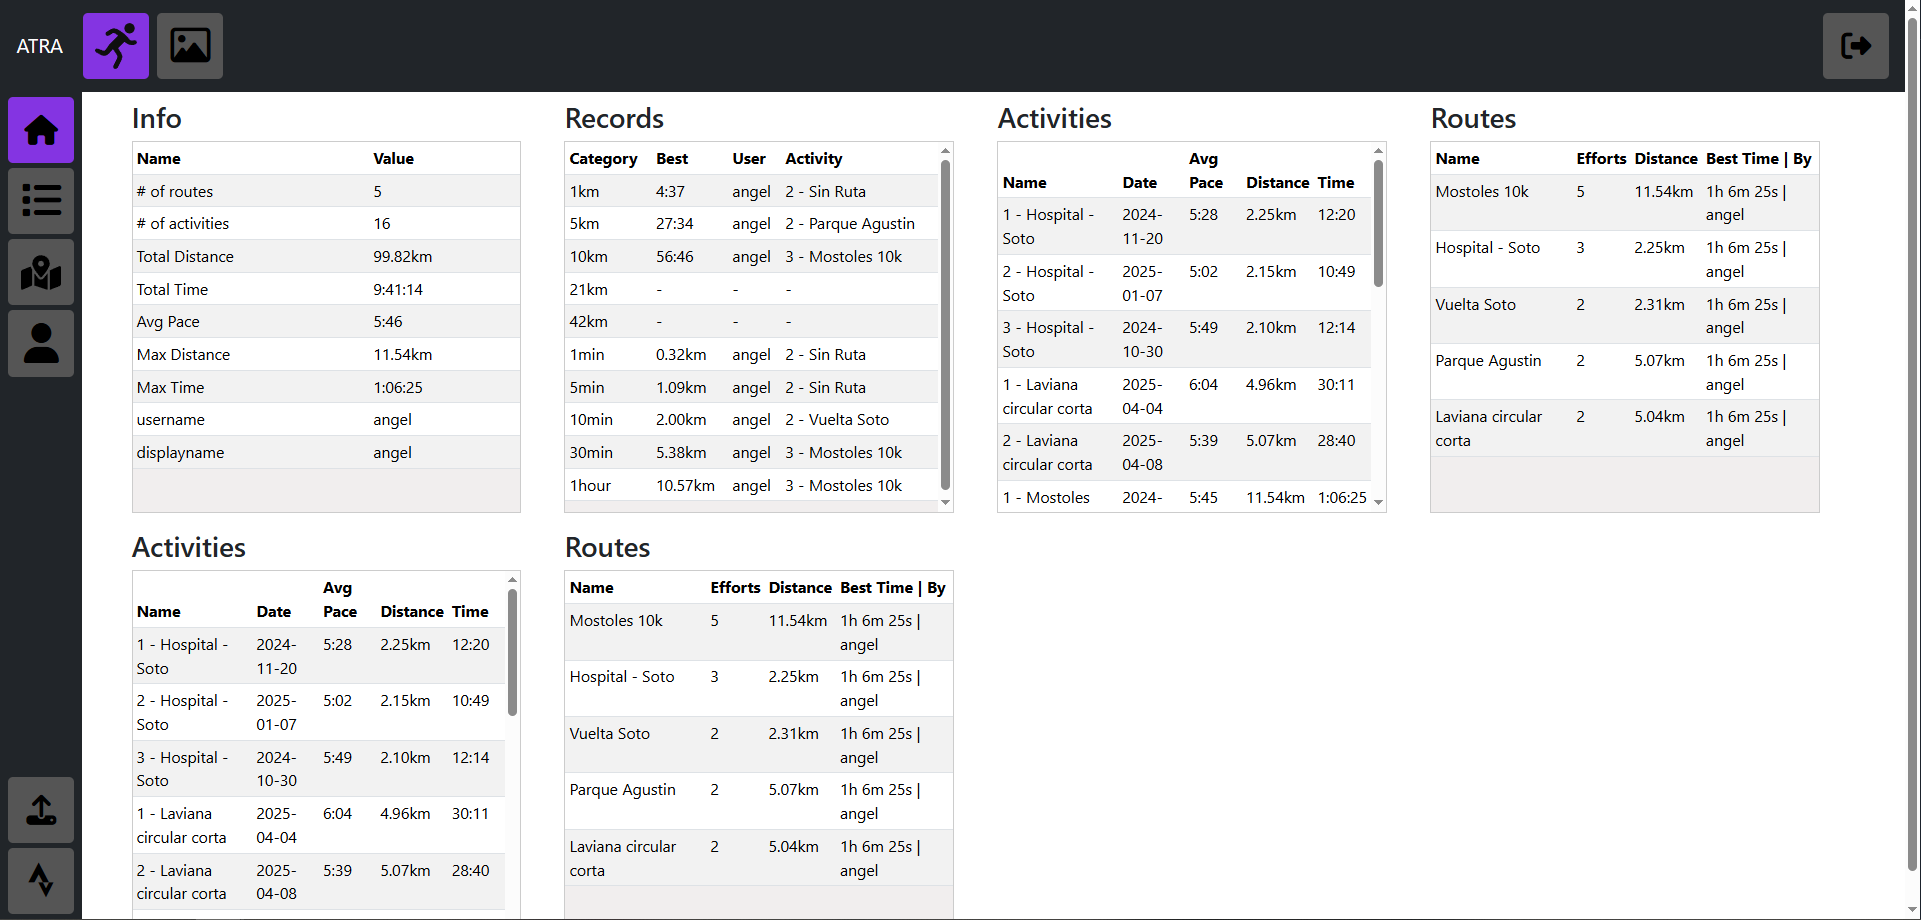
\includegraphics[width=0.75\linewidth]{img/user_dashboard.png}
    \caption{Dashboard de usuario}
    \label{fig:user_dashboard}
\end{figure}
Como se puede ver en la figura, el \textit{dashboard} consiste de los siguientes paneles:
\begin{itemize}
    \item El panel \textbf{info} contiene información general sobre el usuario. Concretamente:
    \begin{itemize}
        \item Número total de rutas y actividades.
        \item Distancia y tiempo total acumulado en todas las actividades creadas.
        \item Ritmo medio a través de todas las actividades.
        \item Distancia máxima recorrida en una única actividad.
        \item Duración máxima de una única actividad.
        \item Nombre público.
        \item Nombre de usuario.
    \end{itemize}
    \item El panel \textbf{Activities} muestra un listado de actividades creadas. Hacer click en una la selecciona para su estudio.
    \item El panel \textbf{Routes} muestra un listado de rutas creadas. Hacer click en una lleva al usuario a la página de rutas, con esta seleccionada, para que pueda visualizar su información.
    \item El panel \textbf{Records} se discute en la sección sobre funcionalidades avanzadas esenciales.
\end{itemize}

Adicionalmente, se puede navegar mediante un menú lateral para acceder al listado de actividades, al listado de rutas, o al perfil de usuario. Dentro del perfil de usuario podrá ver y editar sus datos personales, como su nombre público y dirección de correo electrónico. También podrá editar sus datos de inicio de sesión, siendo estos su nombre de usuario y contraseña, pero hacerlo le forzará a cerrar sesión.

\subsection{Gestión de visibilidad}
La visibilidad no es un recurso de la aplicación como lo son los usuarios, rutas, actividades y murales, sino que es una propiedad que tienen estos recursos (principalmente actividades y rutas). Se ha separado en su propia unidad funcional ya que su implementación implica cierta complejidad. La visibilidad determina si un usuario o mural puede acceder a un recurso. Hay 4 valores posibles: 
\begin{itemize}
    \item Visibilidad \textbf{Privada}: recursos con esta visibilidad sólo son accesibles al usuario que lo ha creado. Nadie más puede ver el recurso ni operar sobre él.
    \item Visibilidad \textbf{Murales Específicos}: recursos con esta visibilidad son visibles para un listado de murales especificados por el creador del recurso (siempre y cuando el creador pertenezca a esos murales). Es posible eliminar o añadir murales a la lista en cualquier momento y sin limitación.
    \item Visibilidad \textbf{Pública a Murales}: recursos con esta visibilidad son visibles para todo aquel mural al que pertenezca el usuario. Si el usuario abandona el mural por cualquier razón, el mural pierde visibilidad del recurso.
    \item Visibilidad \textbf{Pública}: recursos con esta visibilidad son accesibles a cualquier usuario y mural.
\end{itemize}

No todos los recursos pueden tener todos estos valores de visibilidad. Concretamente:
\begin{itemize}
    \item Usuarios: no tienen visibilidad.
    \item Murales: únicamente visibilidad Pública o Privada. Determina si el mural aparece en la lista de "murales a los que no pertenece el usuario". Los murales públicos aparecerán en esa lista, por lo que cualquiera se podrá unir. Los murales privados no aparecerán, y los nuevos miembros sólo podrán acceder mediante el código del mural.
    \item Rutas: hacen uso de las visibilidades pública, privada, y pública a murales.
    \item Actividades: hacen uso de todas las visibilidades.
\end{itemize}

Por defecto todos los recursos son creados con visibilidad Privada, aunque se puede seleccionar otro valor durante la creación. Una vez creado el recurso, depende del tipo de recurso si puede ser editada. La visibilidad de actividades siempre puede ser editada. La visibilidad de una ruta puede ser editada siempre y cuando no sea pública. Hacer una ruta pública fija de manera permanente su visibilidad. La visibilidad de los murales no puede ser cambiada una vez creado el mural.

\section{Funcionalidades avanzadas esenciales}

Las funcionalidades avanzadas esenciales son aquellas que no son necesarias para el funcionamiento básico de la aplicación, pero sin las cuales la experiencia de usar la aplicación no cumpliría los estándares objetivo. Pueden incluir tanto funcionalidades relativamente sencillas, como otras más complejas, o que impliquen integración con sistemas externos.

La mayoría de funcionalidades en esta clasificación tienen que ver con la comparación de actividades.

\subsection{Gestión de actividades}
Las funcionalidades avanzadas esenciales relacionadas con gestión de actividades se centran en la comparación entre actividades. La aplicación permite comparar dos o más actividades independientemente de que estén en la misma ruta o no, y ofrece varias funcionalidades en torno a esta comparación.

Se puede acceder a la funcionalidad de comparación de actividades de dos maneras diferenciadas: desde el listado de actividades, seleccionando varias actividades y pulsando el botón de comparar, o desde la página de rutas, seleccionando comparar las actividades en la ruta seleccionada.

Una vez se accede a la funcionalidad, se muestra un resumen con comparaciones entre las actividades, como cuál es la más larga/corta, cual tiene mayor/menor duración, y cuales tienen el mejor/peor ritmo. Luego, el usuario puede navegar entre varias pestañas (detalladas en las figuras \ref{fig:comparacion_summary}, \ref{fig:comparacion_study}, \ref{fig:comparacion_graphs}, \ref{fig:comparacion_map}):
\begin{itemize}
    \item Summary: contiene las comparaciones descritas, junto con un mapa mostrando todas las actividades.
    \item Study: permite seleccionar una métrica particular, y muestra una serie de medidas estadísticas (las mismas que en estudio de una actividad) para cada una de las actividades seleccionadas, permitiendo su comparación. Adicionalmente, muestra una tabla de récords, y ofrece una calculadora en la que se pueden introducir dos valores de la métrica seleccionada, y muestra, para cada actividad, el porcentaje de valores que caen en la franja determinada.
    \item Graphs: permite seleccionar una métrica particular, y muestra un gráfico de líneas mostrando los valores de cada actividad a lo largo del tiempo.
    \item Map: muestra las actividades en uno o varios mapas. Por defecto muestra tantos mapas como actividades estén siendo comparadas, hasta un máximo de 4. Permite modificar el número de mapas mostrados, aunque nunca se podrán mostrar más mapas que actividades. Permite configurar si cada mapa debe mostrar únicamente la actividad que tiene asignada o si debe mostrar todas. Cuando haya más de 4 actividades en comparación, permite editar qué actividad está siendo mostrada en cada mapa.
\end{itemize}

\begin{figure}[H]
    \centering
    
    % Primera fila
    \begin{minipage}{0.48\linewidth}
        \centering
        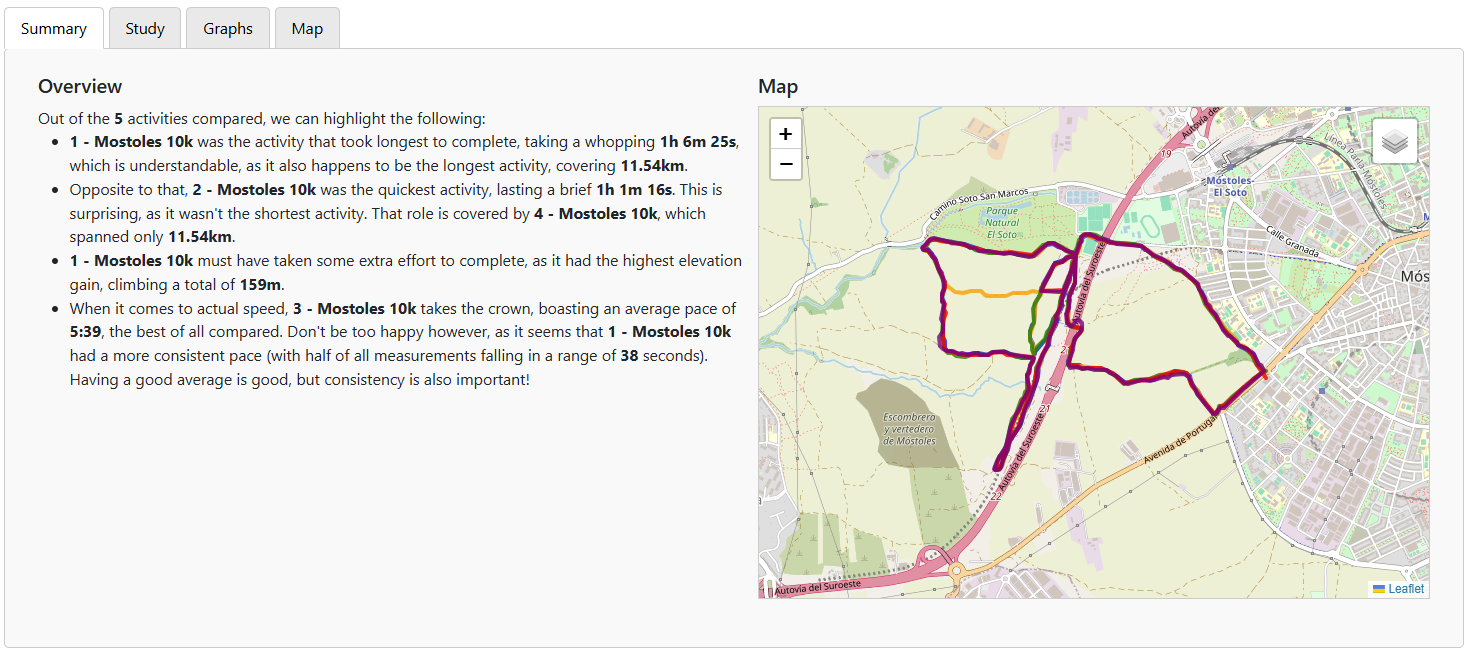
\includegraphics[width=\linewidth]{img/comparacion_summary.png}
        \caption{Resumen de la comparación de actividades}
        \label{fig:comparacion_summary}
    \end{minipage}
    \hfill
    \begin{minipage}{0.48\linewidth}
        \centering
        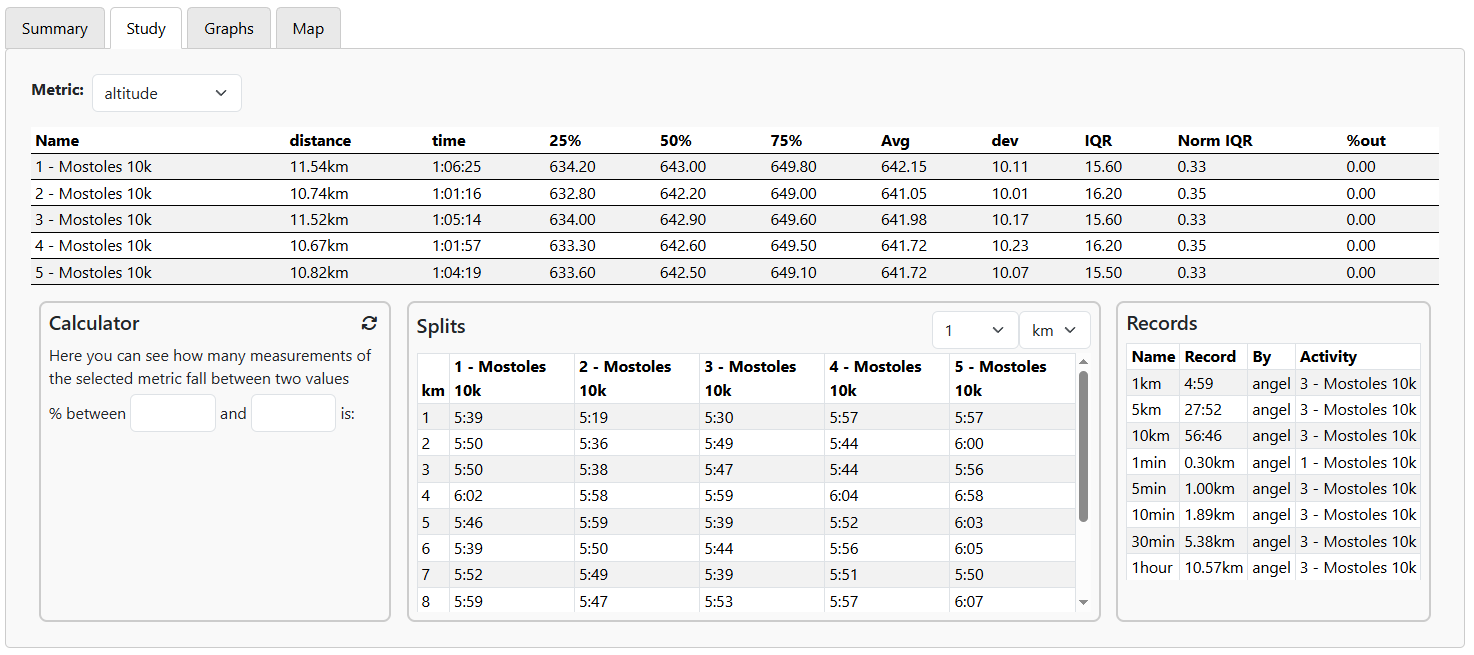
\includegraphics[width=\linewidth]{img/comparacion_study.png}
        \caption{Pestaña de estudio en la comparación de actividades}
        \label{fig:comparacion_study}
    \end{minipage}
    
    \vspace{0.5cm}
    
    % Segunda fila
    \begin{minipage}{0.48\linewidth}
        \centering
        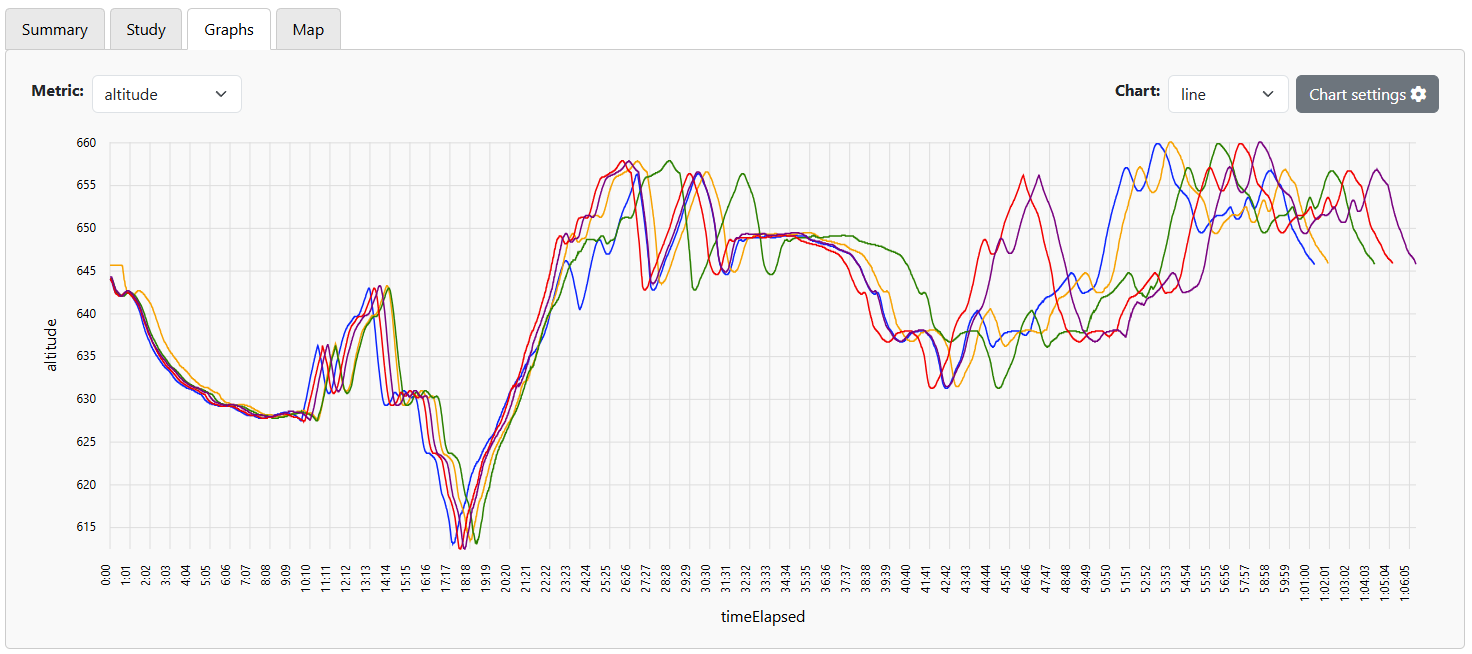
\includegraphics[width=\linewidth]{img/comparacion_graphs.png}
        \caption{Gráficos de comparación de actividades}
        \label{fig:comparacion_graphs}
    \end{minipage}
    \hfill
    \begin{minipage}{0.48\linewidth}
        \centering
        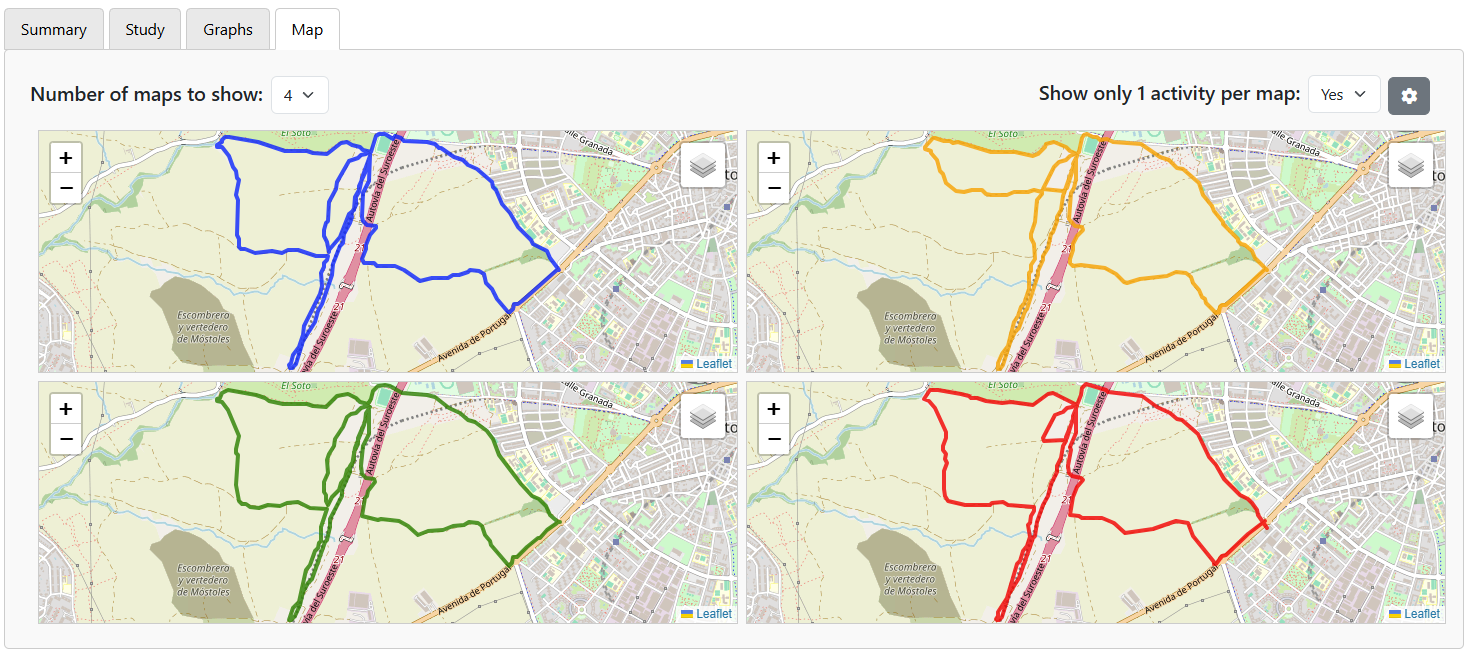
\includegraphics[width=\linewidth]{img/comparacion_map.png}
        \caption{Mapas de actividades en comparación}
        \label{fig:comparacion_map}
    \end{minipage}
    
\end{figure}

\subsection{Gestión de rutas}
Como se ha mencionado en la sección de actividades, la principal funcionalidad avanzada esencial es la comparación de varias actividades en una misma ruta. Esto se ha implementado mediante un botón que aparece junto a los de edición de visibilidad y eliminación de la ruta. Cuando el usuario pulse sobre ese botón, se le muestra un modal listando todas las actividades en la ruta, y permitiéndole seleccionar las actividades que quiera comparar (por defecto están seleccionadas todas las actividades de la ruta). Cuando haya seleccionado las actividades a comparar, será llevado a la página de comparación como si hubiera seleccionado esas actividades manualmente desde la lista de actividades.
\begin{figure}[H]
    \centering
    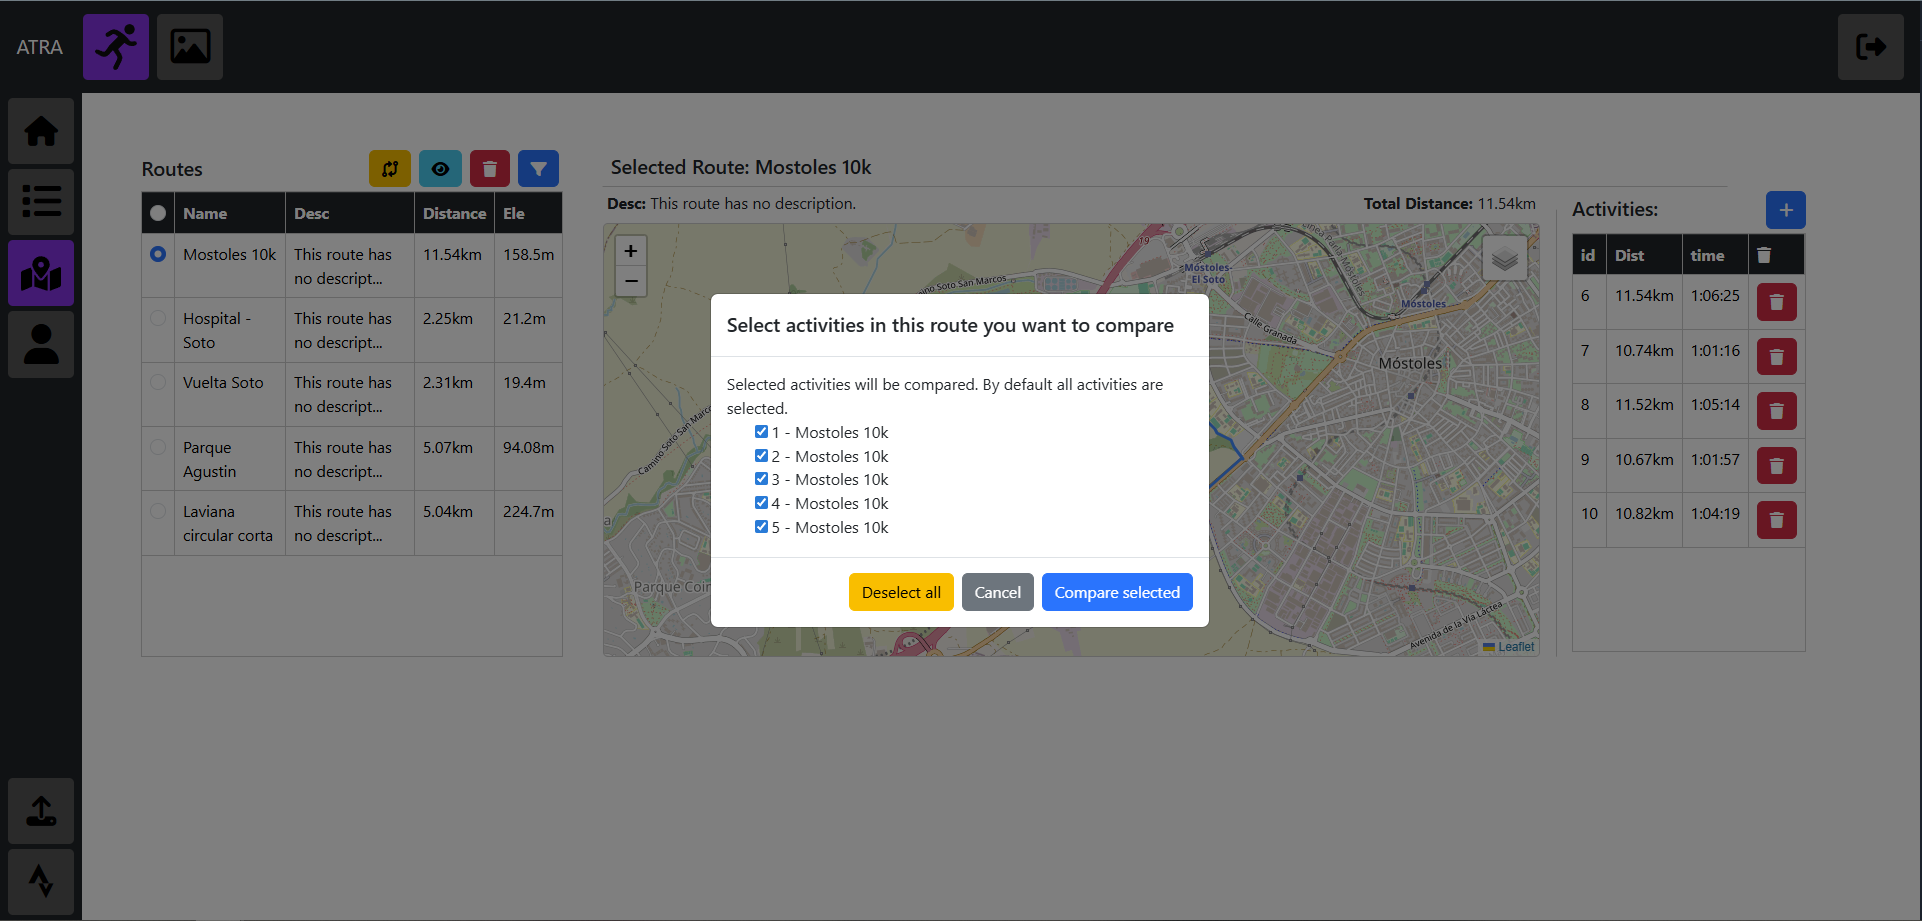
\includegraphics[width=0.75\linewidth]{img/comparar_actividades_ruta.png}
    \caption{Comparación de actividades en la misma ruta}
    \label{fig:placeholder}
\end{figure}

\subsection{Gestión de murales}
En lo referente a la gestión de murales, esta categoría incluye una única funcionalidad: la capacidad para el propietario del mural de banear a usuarios. Un usuario baneado no puede volver a unirse al mural, independientemente de que tenga el código para acceder y de que el mural sea público. Sólo puede volver a unirse al mural si el propietario del mural levanta el baneo.

\subsection{Gestión de usuarios}
Como parte de las funcionalidades avanzadas, se permite a los usuarios ver un listado de récords a través de todas sus actividades. Podrán ver sus mejores marcas para distintas métricas, como mayor distancia recorrida en un tiempo determinado, y menor tiempo usado para cubrir una distancia concreta. Estos récords se muestran en el \textit{dashboard} del usuario como un panel adicional, que consiste en una tabla mostrando: la métrica, la mejor marca obtenida, y la actividad en la que se obtuvo esa marca. Se puede consultar este nuevo panel en la figura \ref{fig:user_dashboard}

\section{Funcionalidades avanzadas optativas}

Las funcionalidades avanzadas optativas son aquellas que no son necesarias para entregar la experiencia objetivo, pero que, aun así, mejoran la experiencia de usuario o añaden funcionalidades útiles o cómodas. Igual que las avanzadas esenciales, pueden incluir funcionalidades más complejas de implementar o que necesiten integración con sistemas externos. Algunas de las funcionalidades originalmente incluidas en esta categoría no han sido implementadas y se plantean como caminos de mejora a futuro. Esta decisión se ha tomado en base a la aportación de cada funcionalidad frente a la complejidad y tiempo que requiere implementarla. En esta sección sólo se discuten las funcionalidades implementadas, las relegadas a mejoras futuras se discuten en la sección de conclusiones y trabajos futuros.

\subsection{Gestión de actividades}
Las funcionalidades de esta categoría ofrecen personalización adicional y mejoras que hacen el uso de la aplicación más conveniente.

Se ha añadido un botón de configuración a la pantalla de gráficas. Al pulsar el botón, se muestra un modal desde el cual el usuario puede cambiar el número de particiones del histograma, así como qué representa el eje x en los gráficos de líneas, pudiendo seleccionar distancia cubierta o tiempo transcurrido. Cuando esté comparando actividades, esta sección también le permitirá decidir qué actividades se deben mostrar en los gráficos, así como seleccionar la estrategia de eliminación de valores duplicados en la gráfica de líneas. Además, se ha añadido la posibilidad de comparar las actividades mediante histogramas. Independientemente de las actividades en comparación, se mostrarán dos histogramas, para asegurar que resulten legibles. Luego, desde la configuración, el usuario tiene la opción de definir qué actividad se debe mostrar en cada histograma. 

\begin{figure}[H]
    \centering
    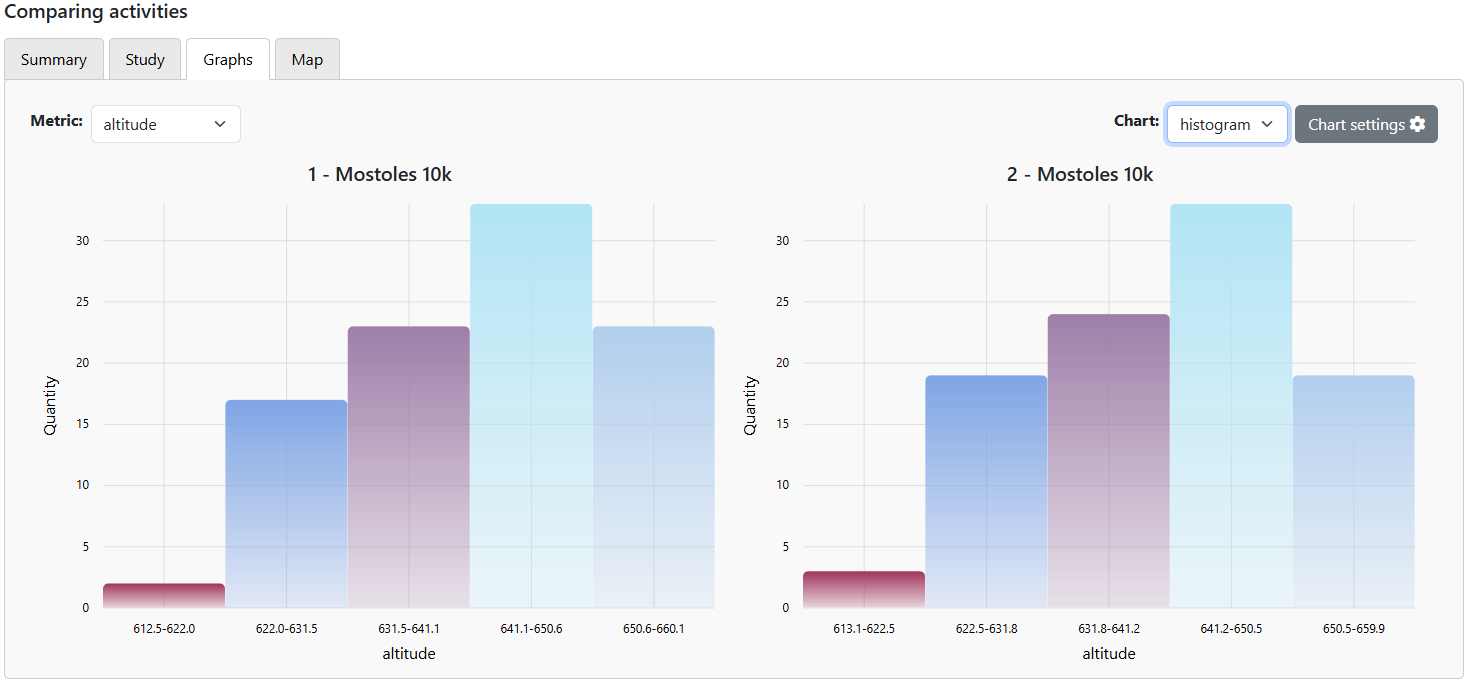
\includegraphics[width=0.75\linewidth]{img/comparacione_histograma.png}
    \caption{Histogramas en comparación de actividades}
    \label{fig:comparacione_histograma}
\end{figure}

La pestaña \textit{Study} también incluye funcionalidad nueva en esta fase. Se ha añadido una herramienta que divide las actividades en particiones de distancia fija y muestra el ritmo medio de cada actividad en cada división. Ofrece valores fijos para las particiones (1km, 5km...), pero también permite hacer divisiones de longitud establecida por el usuario. Además, permite cambiar la unidad de medida entre kilómetros y millas, aunque el ritmo siempre se muestra en minutos por kilómetro. Esta funcionalidad se puede ver en la figura \ref{fig:comparacion_study}.

Por último, se ha añadido una funcionalidad de calidad de vida en la selección de actividades. Al mantener el cursor sobre una actividad en el listado de actividades un tiempo determinado, aparece un \textit{popover} mostrando un mapa con la actividad, para facilitar su identificación. 

\subsection{Gestión de rutas}
En gestión de rutas se incluye una funcionalidad de  mejora de usabilidad, que permite filtrar el listado de rutas en función de su visibilidad. Esto permite a los usuarios reducir el tamaño de la lista, de forma que sea más fácil de gestionar cuando existan muchas rutas.

\subsection{Gestión de murales}
Dentro de gestión de murales, se inlcuye una funcionalidad que permite a los propietarios de un mural traspasar el rol de propietario a otro usuario. Cuando haga esto, pasará a ser un miembro normal, perdiendo acceso a todas las funcionalidades a las que tiene acceso como propietario, y el usuario seleccionado pasará a ser el nuevo propietario con acceso a esas funcionalidades. Además, esto permite que el propietario de un mural abandone el mismo. Al pulsar el botón de abandonar mural, se le permite elegir un sucesor. Si no lo elige, se elegirá uno automáticamente.
\begin{figure}[H]
    \centering
    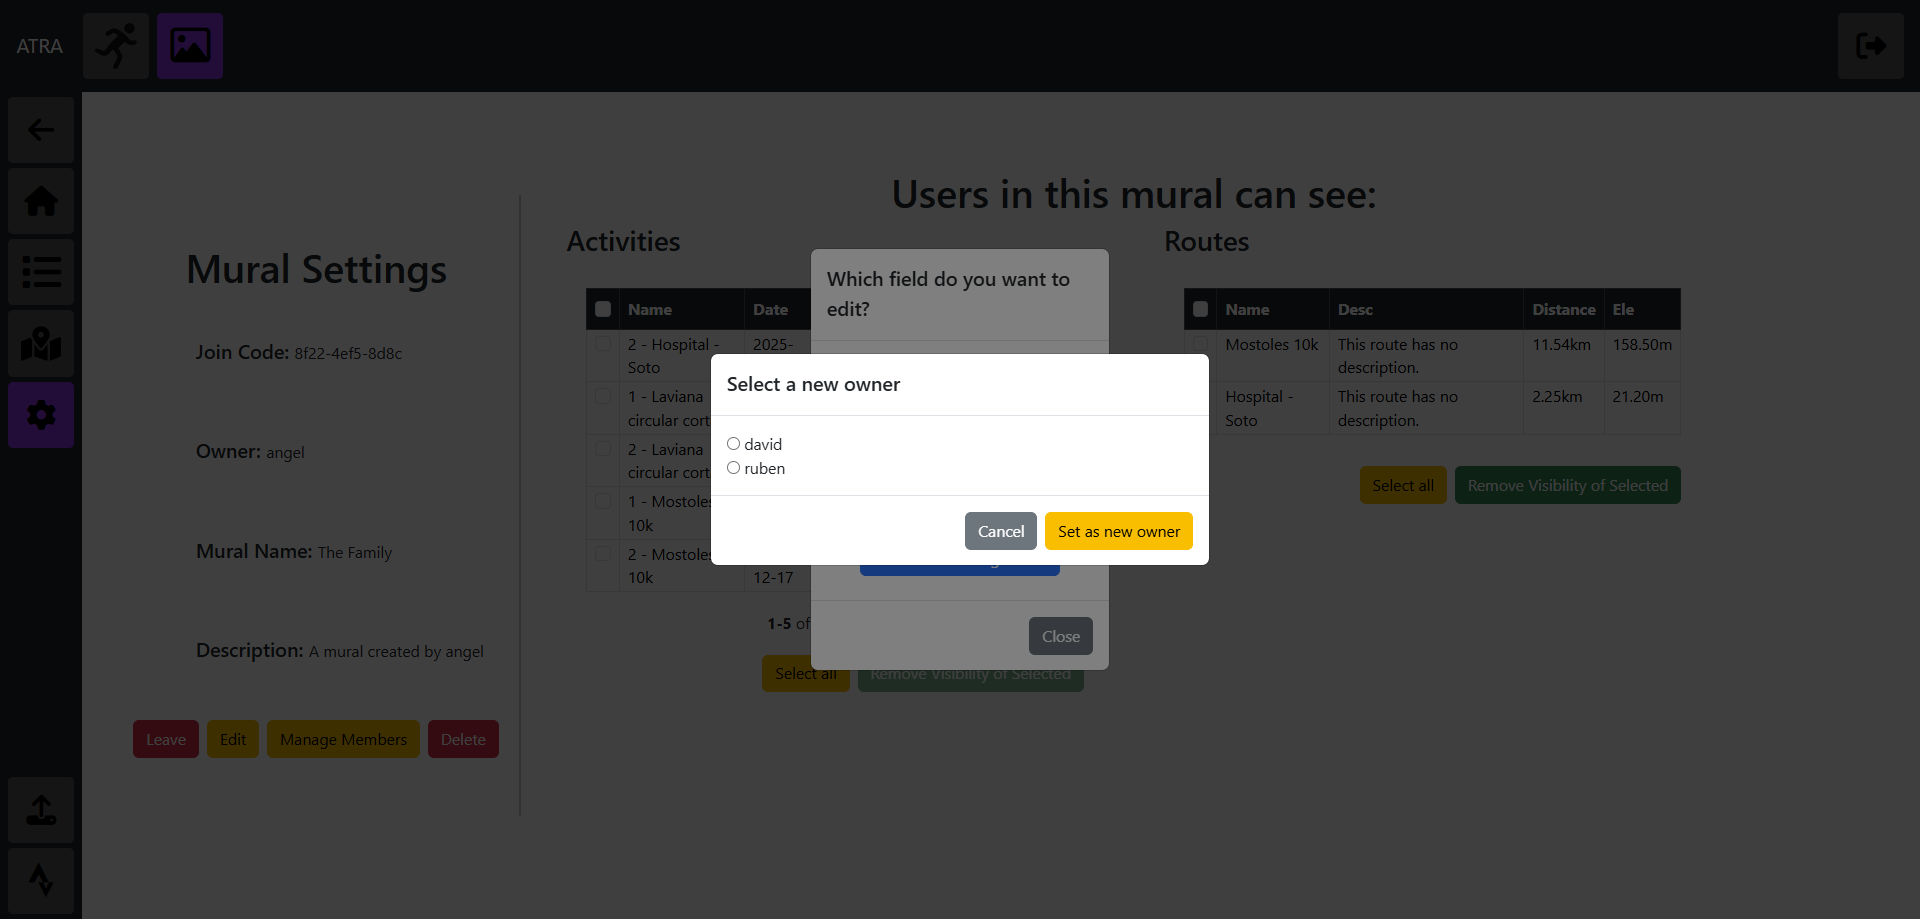
\includegraphics[width=0.75\linewidth]{img/cambiar_owner.png}
    \caption{Cambio de propietario de mural}
    \label{fig:placeholder}
\end{figure}